\chapter[Desenvolvimento]{Desenvolvimento}
\label{ch:desenvolvimento}
O \textit{Power Monitor} surgiu da necessidade da conscientização do gasto energético e da melhor compreensão da conta de luz. Baseado nesse conceito,
foi desenvolvido um \textit{software} que permite uma fácil comunicação com qualquer equipamento construído que tenha a finalidade de monitorar a energia elétrica. 
O sistema traz uma forma mais fácil e próxima do consumidor final de quantificar a energia elétrica consumida em um estabelecimento. No lugar do Quilowatt-hora, medida que é usada atualmente,
o \textit{software} propõe mensurar o gasto energético em reais (R\$), trazendo a realidade do consumo mensal para mais próximo de cada brasileiro.

Nesse capítulo será mostrado todo o passo a passo para o desenvolvimento do \textit{software} e \textit{hardware}, juntamente com a comunicação 
entre ambos. 


\section[\textit{Visão Geral}]{\textit{Visão Geral}}\label{visal-geral}

Em resumo pode-se ter uma visão geral de como o ambiente - \textit{software} e \textit{hardware} - funciona observando a \autoref{fig:diagrama-vg}.
O sistema \textit{web} é responsável por fazer a comunicação entre o banco de dados e os dispositivos, já os eletrodomésticos são gerenciados
pelo NodeMCU que possui uma comunicação direta via \textit{websocket} com o servidor \textit{web}.

\begin{figure}[h!]
	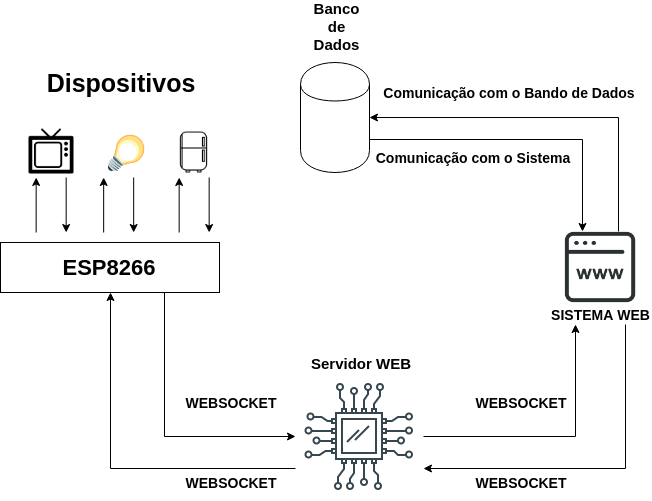
\includegraphics[width=0.7\textwidth, keepaspectratio=true]{diagrama-1}
	\centering
	\caption[Visão geral do ambiente]{Visão geral do ambiente}
	\label{fig:diagrama-vg}
\end{figure}
\FloatBarrier

\section[\textit{Software}]{\textit{Software}}\label{soft-sec}
O controle dos dispositivos de um cômodo, que estão interligados com o \textit{NodeMCU} são controlados pelo \textit{software}. Dessa forma
todos os dispositivos que possuem comunicação com a plataforma de prototipagem e que estão cadastrados nos sistema podem ser controlados (Ligar/Desligar) e também
é possível ter um acompanhamento dos gastos.

O sistema possui uma interface \textit{web} que pode ser acessada por qualquer dispositivo que tenha acesso a internet e possua um 
\textit{browser}, como por exemplo: celulares, computadores, \textit{smart tv} etc. O \textit{software} possui uma interface de apenas um único usuário, ao acessar o sistema o usuário se depara com um
visual bem agradável e fácil de se usar. Logo ao entrar no sistema o utente se depara com a tela principal, \autoref{fig:principal-ft}, nela encontra-se
as principais informações que o usuário irá precisar, como também irá mostrar as opções de cadastrar um novo dispositivo, listar os dispositivos, cadastrar um novo cômodo,
listar um novo cômodo etc.

\begin{figure}[h!]
	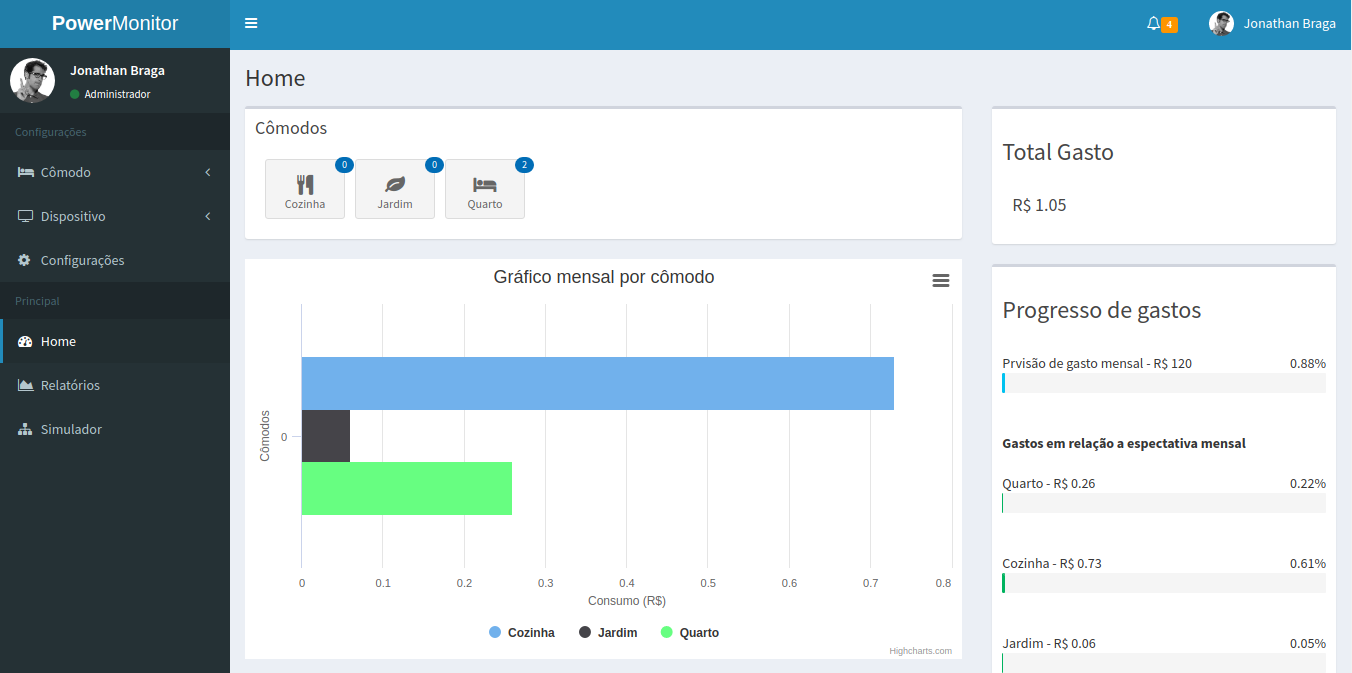
\includegraphics[width=1.0\textwidth, keepaspectratio=true]{principal}
	\centering
	\caption[Tela inicial do sistema]{Tela inicial do sistema}
	\label{fig:principal-ft}
\end{figure}
\FloatBarrier

Todas as informações colhidas pelo servidor \textit{web} em \textit{node.js} (\autoref{node}), são recebidas e tratadas pelo interface \textit{web}. Os dados
são importantíssimos, pois mediante eles é que se torna possível a construção dos gráficos e das previsões fornecidas pelo sistema. No \textit{power monitor}
a forma de comunicação com o banco de dados é feita mediante as chamadas de API, existe uma chamada para cada ação prevista no sistema. A \autoref{fig:api-ft}
retrata bem esse cenário, pode-se perceber que o \textit{end-point} (expressão utilizada para se referenciar a uma extremidade de um canal de comunicação.) 
\textbf{get-comodos} é destinado a obtenção de todos os cômodos cadastrados já o \textit{end-point} \textbf{get-dispositivos} é destinado a 
obtenção de todos os dispositivos cadastrados. O motivo da comunicação entre servidor \textit{web} e interface \textit{web}
ser feita via chamada de API é bem simples, pois qualquer sistema seja \textit{web, desktop} ou qualquer outro tipo, pois basicamente precisa ter uma comunicação com uma rede \textit{Wi-Fi}
para utilizar o \textit{power monitor}. O \textit{software} não precisa obrigatoriamente de internet para poder funcionar, pois a comunicação entre servidor e sistema é
baseada em uma rede local, justamente para que o \textit{software} não dependa de terceiros. Para uma perfeita comunicação o ambiente só precisa está configurado
na mesma rede \textit{Wi-Fi}. 

\begin{figure}[h!]
	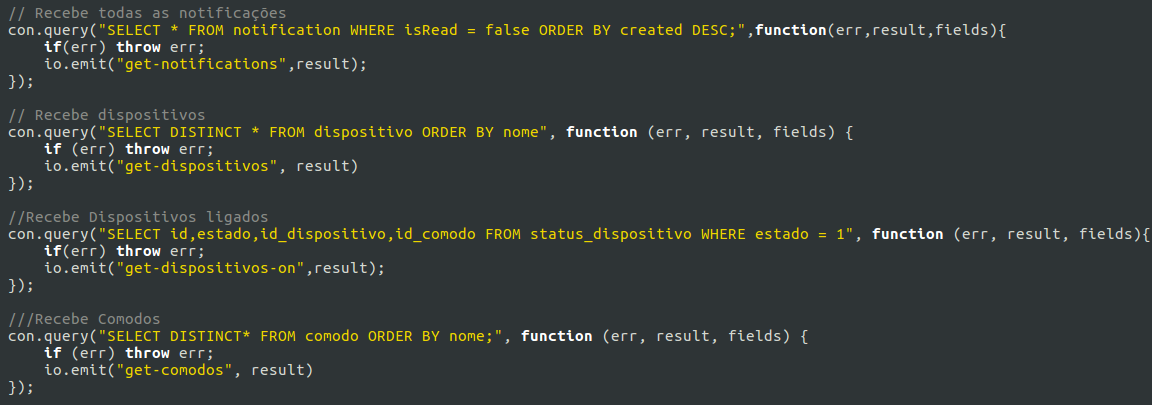
\includegraphics[width=1.0\textwidth, keepaspectratio=true]{api}
	\centering
	\caption[Chamada de API]{Chamada de API}
	\label{fig:api-ft}
\end{figure}
\FloatBarrier

O \textit{software} pode ser dividido em duas partes, servidor \textit{web} e interface \textit{web}. O servidor foi desenvolvido usando a linguagem
\textit{javascript} (\autoref{js}) e para auxílio foi utilizado o \textit{framework node.js} (\autoref{node}), a comunicação entre servidor e banco de dados
é feita pelo \textit{MySQL Server} (\autoref{sql}). A interface \textit{web} é o agente consumidor de todos esses serviços, com uma comunicação via 
\textit{webscoket} (\autoref{websocket}) com o servidor é capaz de receber e enviar dados a todo instante. A combinação desses três serviços - servidor \textit{web},
servidor do banco de dados e interface \textit{web} - resultou em uma aplicação intuitiva e amigável, desenvolvida para dar o total suporte às análises dos dados
enviados pelo \textit{hardware}. A \autoref{fig:banco-dados} representa o esquema das tabelas do banco de dados que foi utilizado no \textit{power monitor}.

Como já foi apresentada a \autoref{fig:principal-ft} representa a tela inicial da interface \textit{web}, vê-se que é possível
visualizar o total gasto no mês atual, o progresso dos gastos por cômodo que por sua vez é baseado na expectativa de gasto mensal (\autoref{fig:configuracao-ft}), a lista
de todos os cômodos cadastrados e um gráfico mostrando o consumo por cômodo referente ao mês atual.

\begin{figure}[h!]
	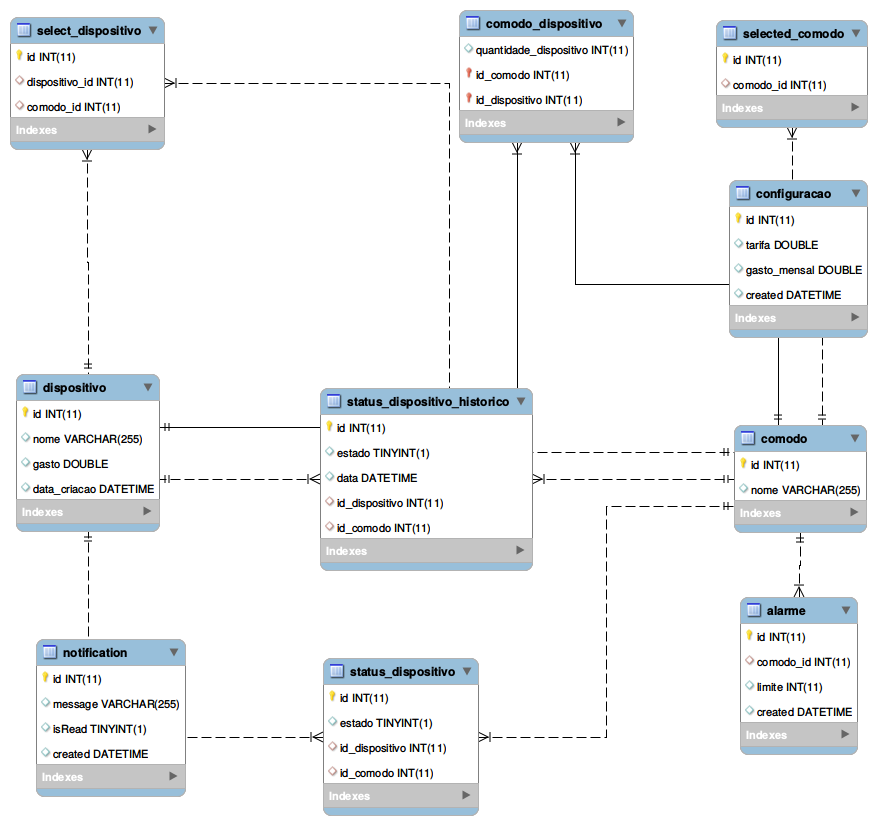
\includegraphics[width=1.0\textwidth, keepaspectratio=true]{banco}
	\centering
	\caption[Esquema das tabelas do banco de dados]{Esquema das tabelas do banco de dados}
	\label{fig:banco-dados}
\end{figure}
\FloatBarrier

As figuras: \ref{fig:c-comodo}, \ref{fig:l-comodo}, \ref{fig:c-dispositivo}, \ref{fig:l-dispositivo} e \ref{fig:configuracao-ft}, 
são relacionadas as telas de cadastro, listagem e de configuração da interface \textit{web}. Nelas é possível cadastrar e listar comôdos e dispositivos assim como 
configurar alguns parâmetros do sistema como o preço da tarifa cobrada por quilowatt-hora pela empresa responsável e a expectativa de gasto mensal.

Uma vez que os cômodos, dispositivos e parâmetros são cadastrados no sistema é possível gerencia-los através da edição ou exclusão dos dados, que se torna possível
nas telas de listagem, para os cômodos e dispositivos, já os parâmetros do sistema na própria tela de configuração se faz a edição dos dados. 

\begin{figure}[h!]
	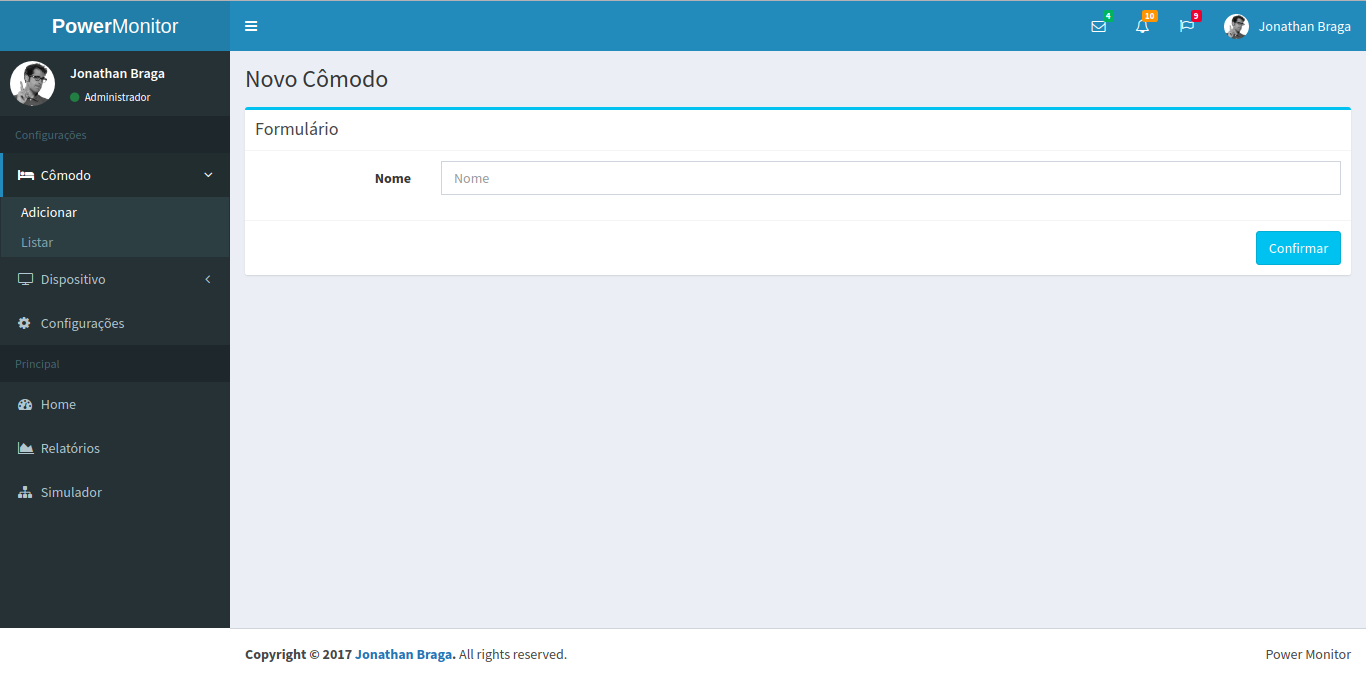
\includegraphics[width=1.0\textwidth, keepaspectratio=true]{c-comodo}
	\centering
	\caption[Cadastro de um cômodo]{Cadastro de um cômodo}
	\label{fig:c-comodo}
\end{figure}
\FloatBarrier

\begin{figure}[h!]
	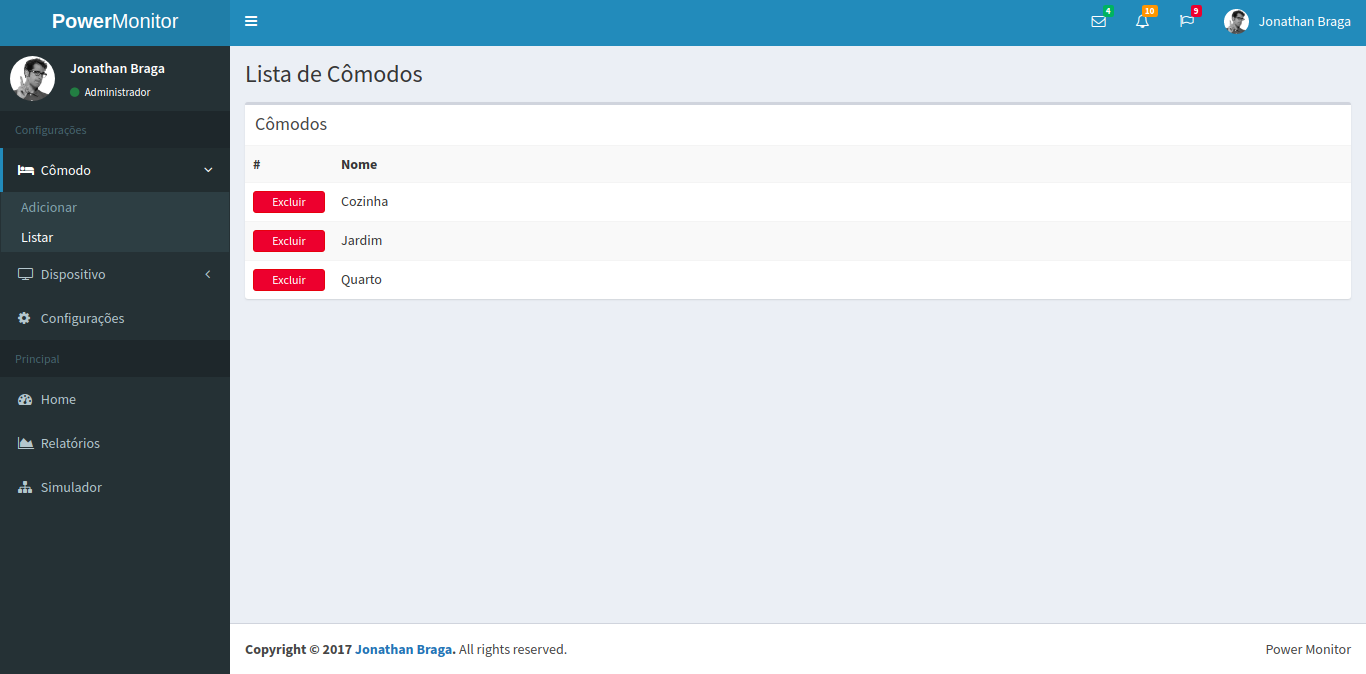
\includegraphics[width=1.0\textwidth, keepaspectratio=true]{l-comodo}
	\centering
	\caption[Lista dos cômodos cadastrados]{Lista dos cômodos cadastrados}
	\label{fig:l-comodo}
\end{figure}
\FloatBarrier

\begin{figure}[h!]
	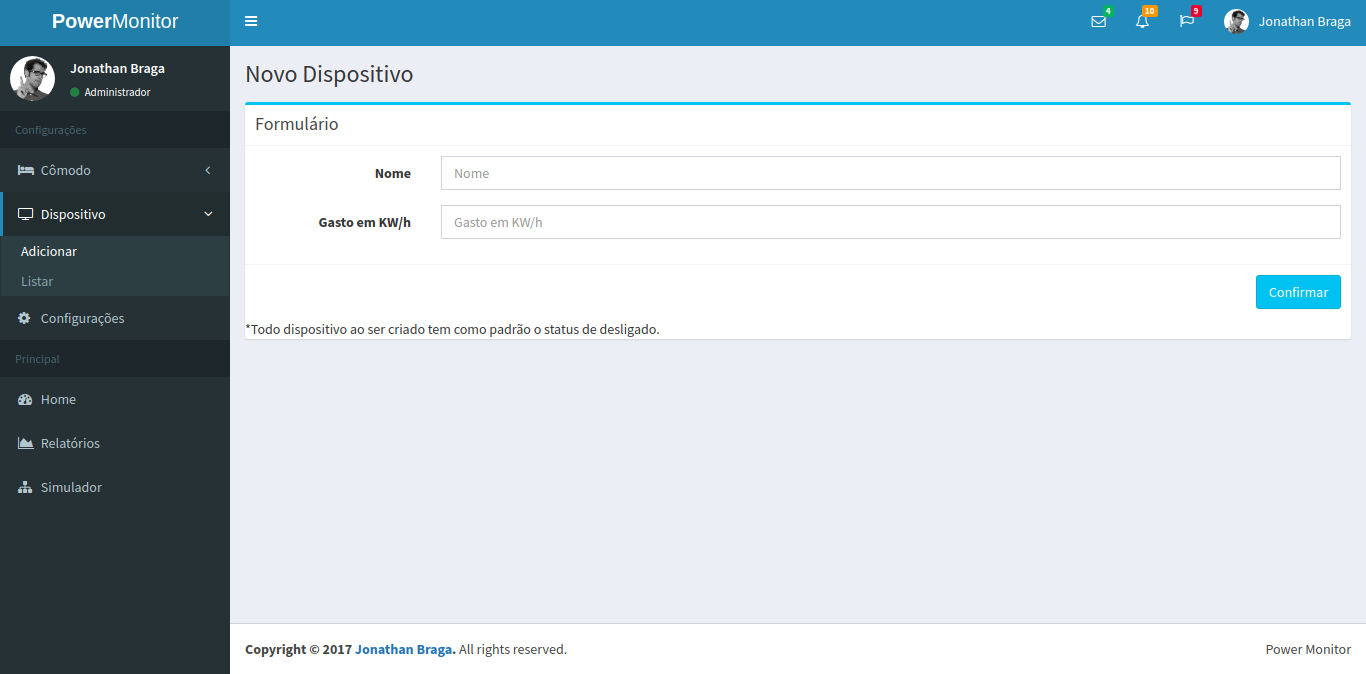
\includegraphics[width=1.0\textwidth, keepaspectratio=true]{c-dispositivo}
	\centering
	\caption[Cadastro de um dispositivo]{Cadastro de um dispositvio}
	\label{fig:c-dispositivo} 
\end{figure}
\FloatBarrier

\begin{figure}[h!]
	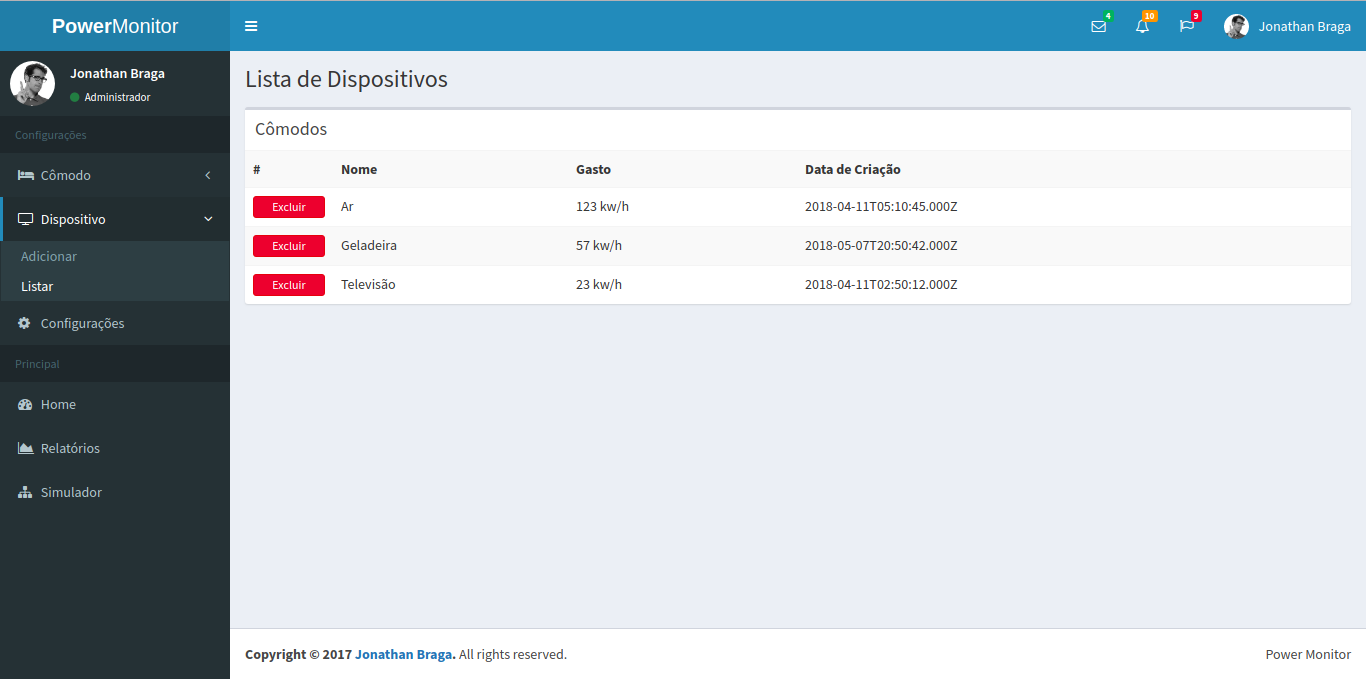
\includegraphics[width=1.0\textwidth, keepaspectratio=true]{l-dispositivo}
	\centering
	\caption[Listagem dos dispositivos cadastrados]{Listagem dos dispositivos cadastrados}
	\label{fig:l-dispositivo} 
\end{figure}
\FloatBarrier

\begin{figure}[h!]
	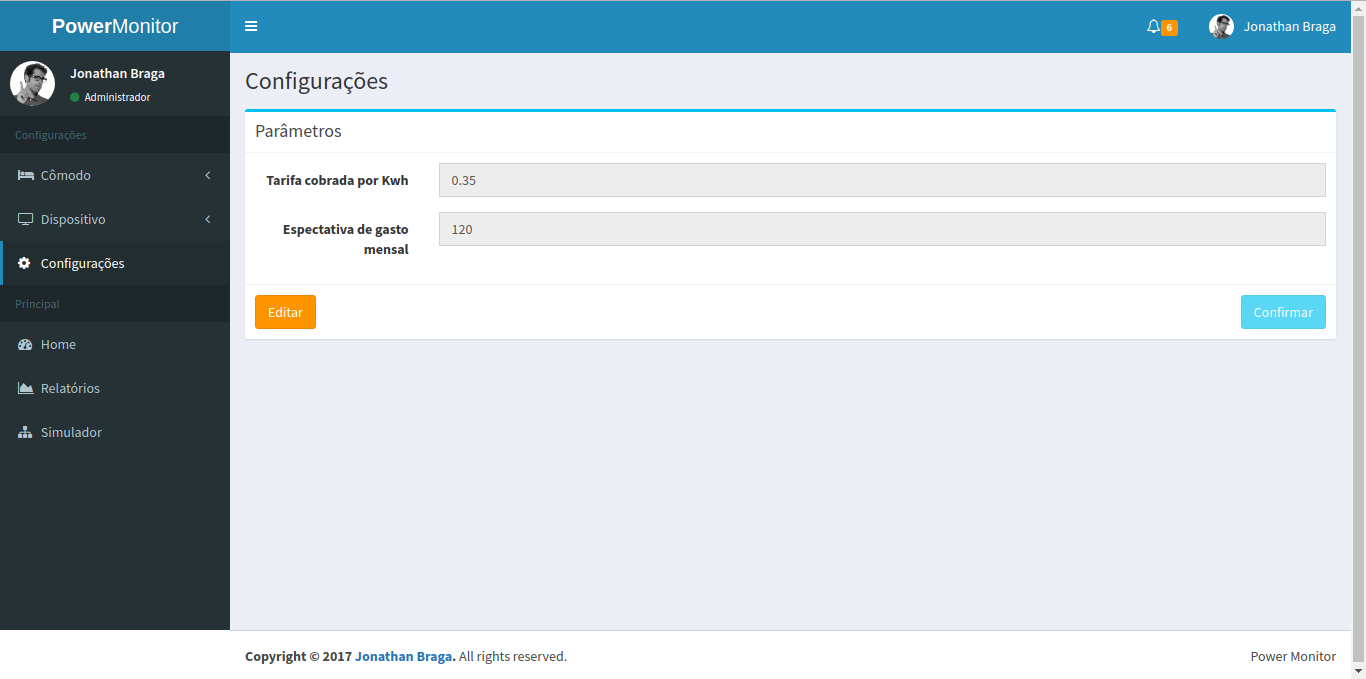
\includegraphics[width=1.0\textwidth, keepaspectratio=true]{configuracao}
	\centering
	\caption[Tela de configuração dos parâmetros do sistema]{Tela de configuração dos parâmetros do sistema}
	\label{fig:configuracao-ft} 
\end{figure}
\FloatBarrier

Uma vez que todos os cômodos, dispositivos e parâmetros já se encontram cadastrados e já exista a comunicação estabelecida com o hardware, a interface
\textit{web} disponibiliza um séria de formas para visualização das informações coletadas e tratadas. Na \autoref{fig:extrato} é possível visualizar
uma espécie de extrato do consumo de todos os dispositivos, podendo perceber quando foram ligados, quando foram desligados e assim resultando no total gasto.
Já as figuras: \ref{fig:ano-c}, \ref{fig:matu-c} e \ref{fig:mant-c} referem-se aos gráficos que são construídos baseados nas informações coletadas pelo sistema.

Os gráficos por sua vez são construídos mediante aos cálculos que o sistema faz usando como base a \autoref{eq-consumo}, o resultado dessa conta
fornece ao sistema o consumo em reais (R\$) do dispositivo em um dado intervalo de tempo conhecido. Vale salientar que o resultado é o esperado já que o consumo
do dispositivo (KWh) é pré definido pelo usuário (\autoref{fig:c-dispositivo}), para o cálculo real do consumo usa-se a \autoref{eq-potencia} que leva em conta a corrente real que passa
pelo dispositivo ao longo do tempo que ele permanece ligado. Com esses dados é que se torna viável a construção dos gráficos e extrato presentes no sistema.

\begin{equation} \label{eq-consumo}
	\frac{consumo \, \, do \, \, dispositivo \times tempo \, \, de \, \, uso}{número \, \, de \, \, dias \, \, no \, \, mês} \times tarifa
\end{equation}

\begin{equation} \label{eq-potencia}
	 \frac{ (tensão \times corrente) \times horas \, \, de \, \, uso \, \, por dia \times número \, \, de \, \, dias \, \, no \, \, mês}{1000}
\end{equation} 

\begin{figure}[h!]
	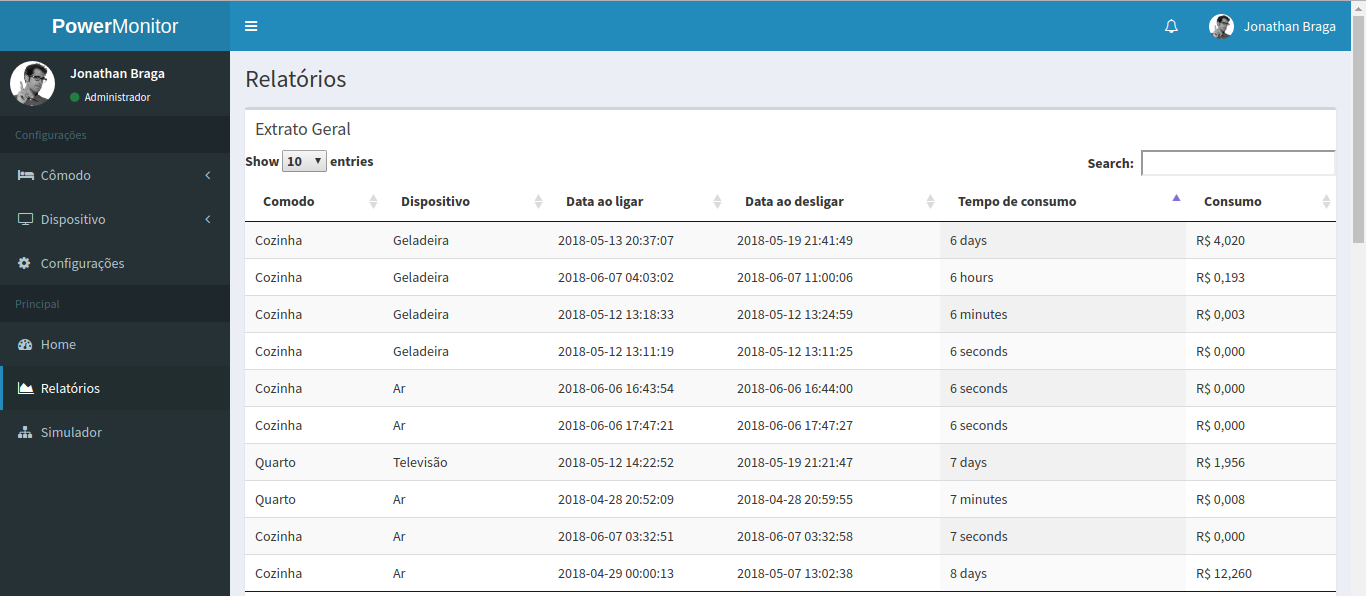
\includegraphics[width=1.0\textwidth, keepaspectratio=true]{extrato}
	\centering
	\caption[Demonstrativo do gasto de cada dispositivo]{Demonstrativo do gasto de cada dispositivo}
	\label{fig:extrato} 
\end{figure}
\FloatBarrier

\begin{figure}[h!]
	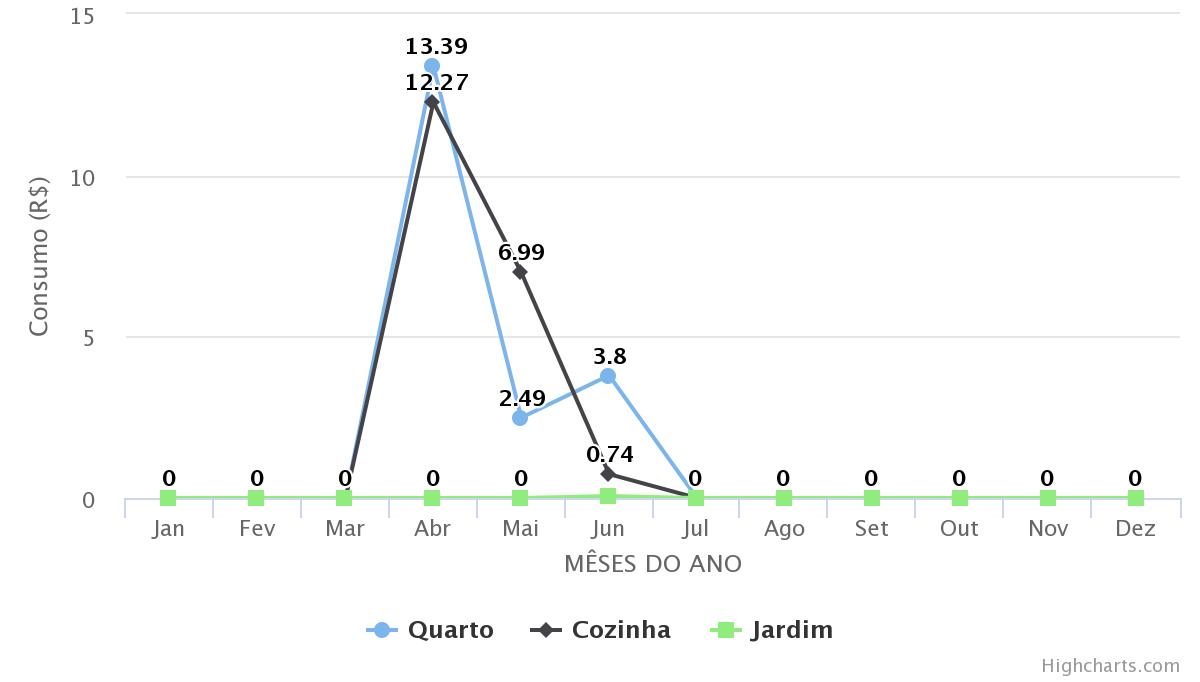
\includegraphics[width=1.0\textwidth, keepaspectratio=true]{ano-c}
	\centering
	\caption[Consumo geral de todos os dispositivos por cômodo ao longo do ano]{Consumo geral de todos os dispositivos por cômodo ao longo do ano}
	\label{fig:ano-c} 
\end{figure}
\FloatBarrier

\begin{figure}[h!]
	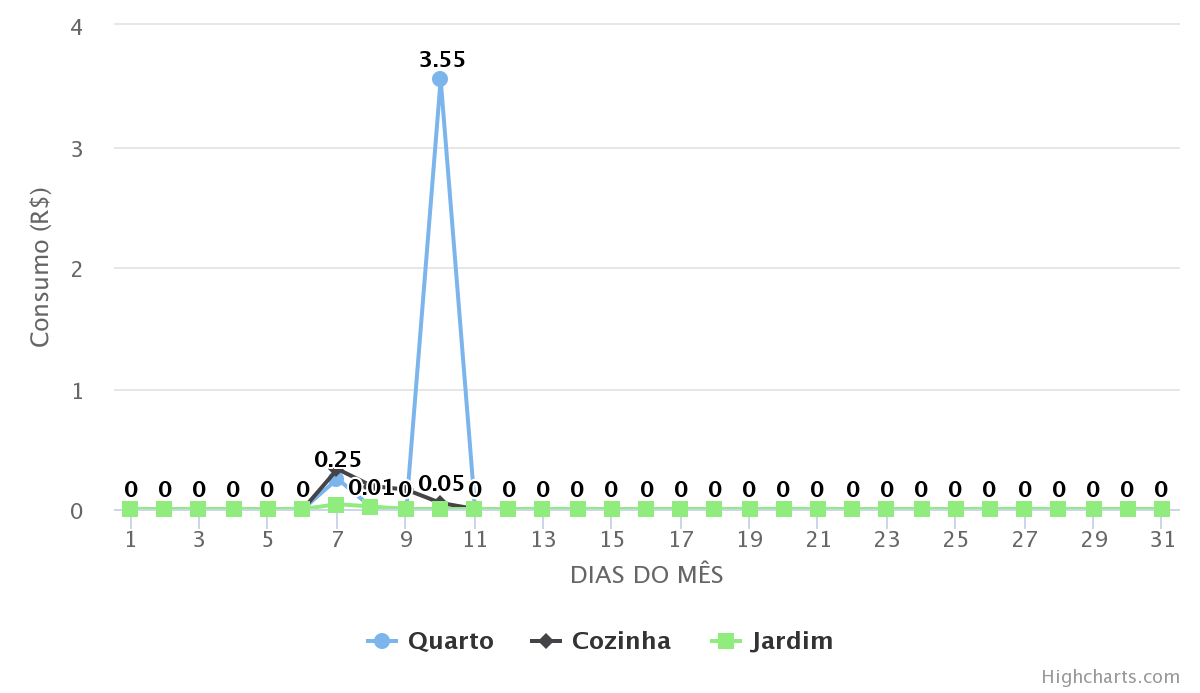
\includegraphics[width=1.0\textwidth, keepaspectratio=true]{matu-c}
	\centering
	\caption[Consumo geral de todos os dispositivos por cômodo ao longo do mês atual]{Consumo geral de todos os dispositivos por cômodo ao longo do mês atual}
	\label{fig:matu-c} 
\end{figure}
\FloatBarrier

\begin{figure}[h!]
	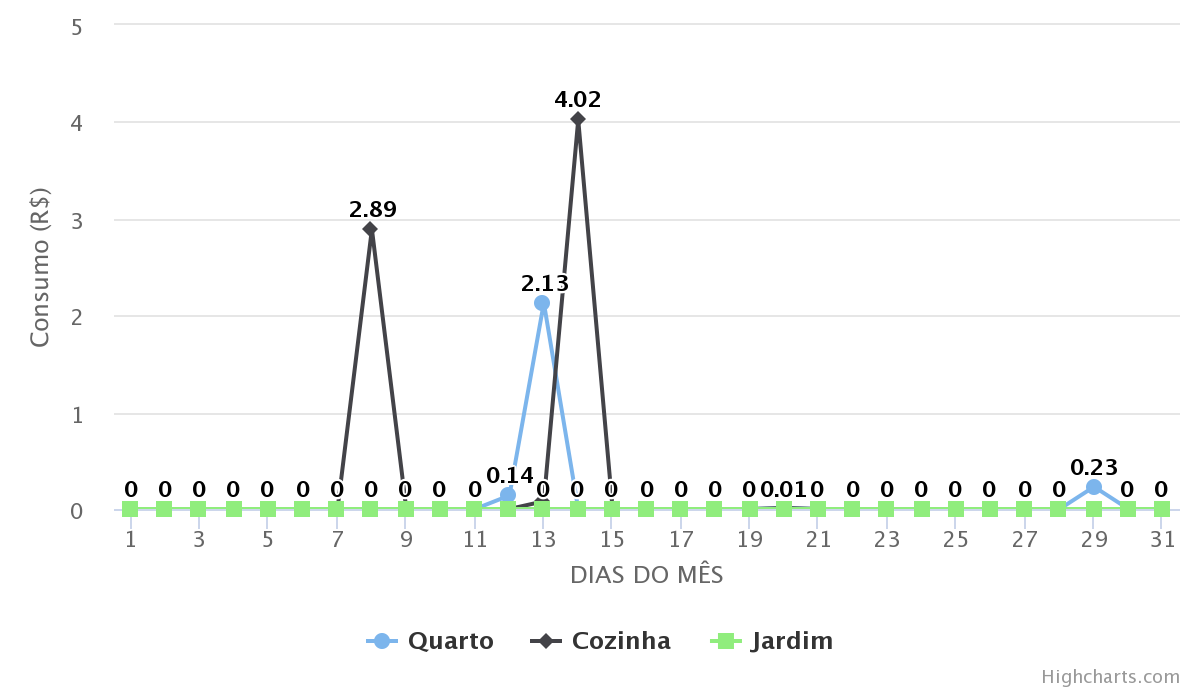
\includegraphics[width=1.0\textwidth, keepaspectratio=true]{mant-c}
	\centering
	\caption[Consumo geral de todos os dispositivos por cômodo ao longo do mês anterior]{Consumo geral de todos os dispositivos por cômodo ao longo do mês anterior}
	\label{fig:mant-c} 
\end{figure}
\FloatBarrier

O \textit{software} também possui um local específico para a gerência dos cômodos, um espaço destinado para a vinculação de dispositivos ao cômodo,
visualização do total gasto em relação ao mês atual em forma de gráfico e a opção de ligar, desligar ou excluir o dispositivo do cômodo. As figuras:
\ref{fig:comodo-ft}, \ref{fig:v-dispositivo} e \ref{fig:a-dispositivo} retratam o cenário descrito.

\begin{figure}[h!]
	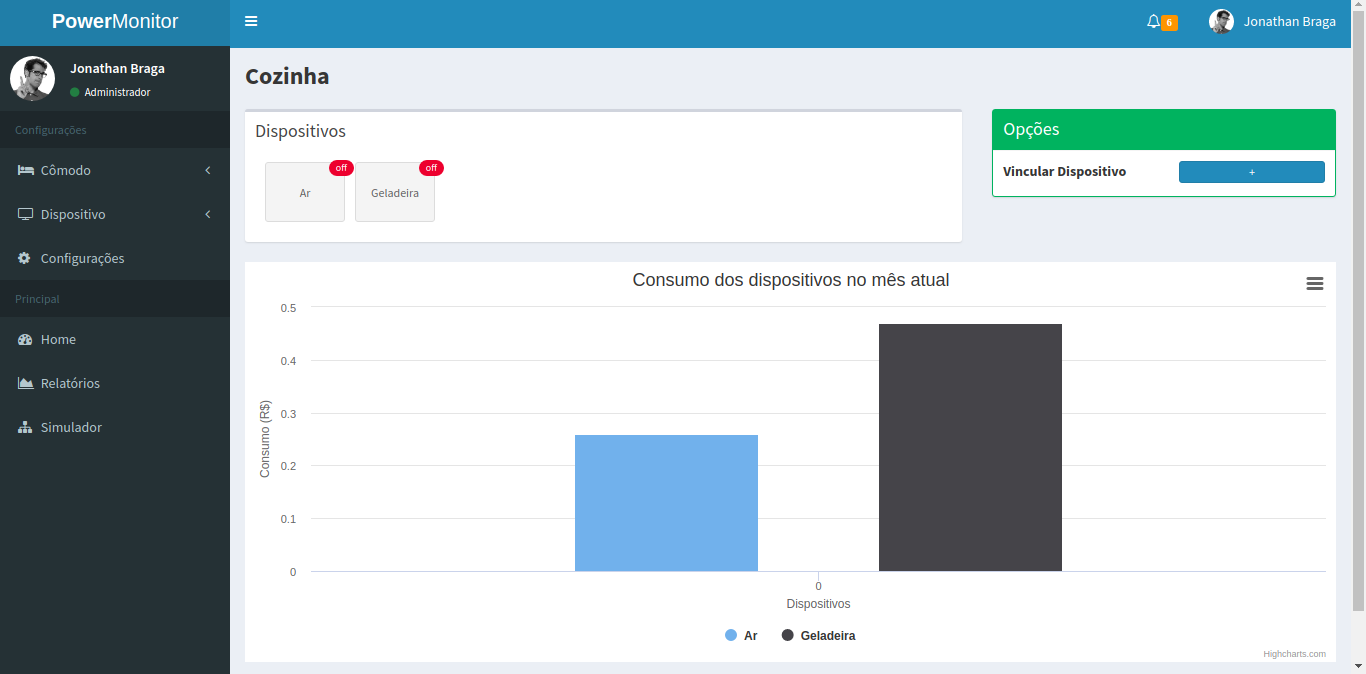
\includegraphics[width=1.0\textwidth, keepaspectratio=true]{comodo}
	\centering
	\caption[Visão geral da gerência de um cômodo]{Visão geral da gerência de um cômodo}
	\label{fig:comodo-ft} 
\end{figure}
\FloatBarrier

\begin{figure}[h!]
	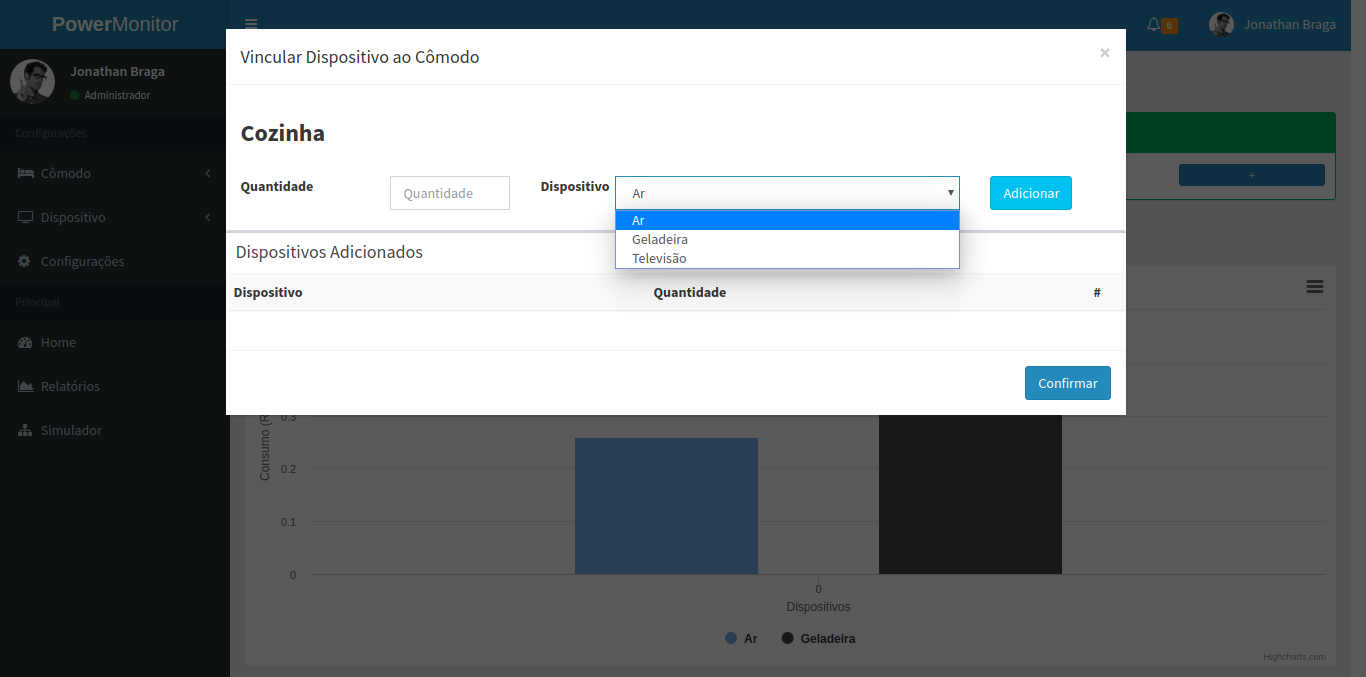
\includegraphics[width=1.0\textwidth, keepaspectratio=true]{v-dispositivo}
	\centering
	\caption[Vincular dispositivo ao cômodo]{Vincular dispositivo ao cômodo}
	\label{fig:v-dispositivo} 
\end{figure}
\FloatBarrier

\begin{figure}[h!]
	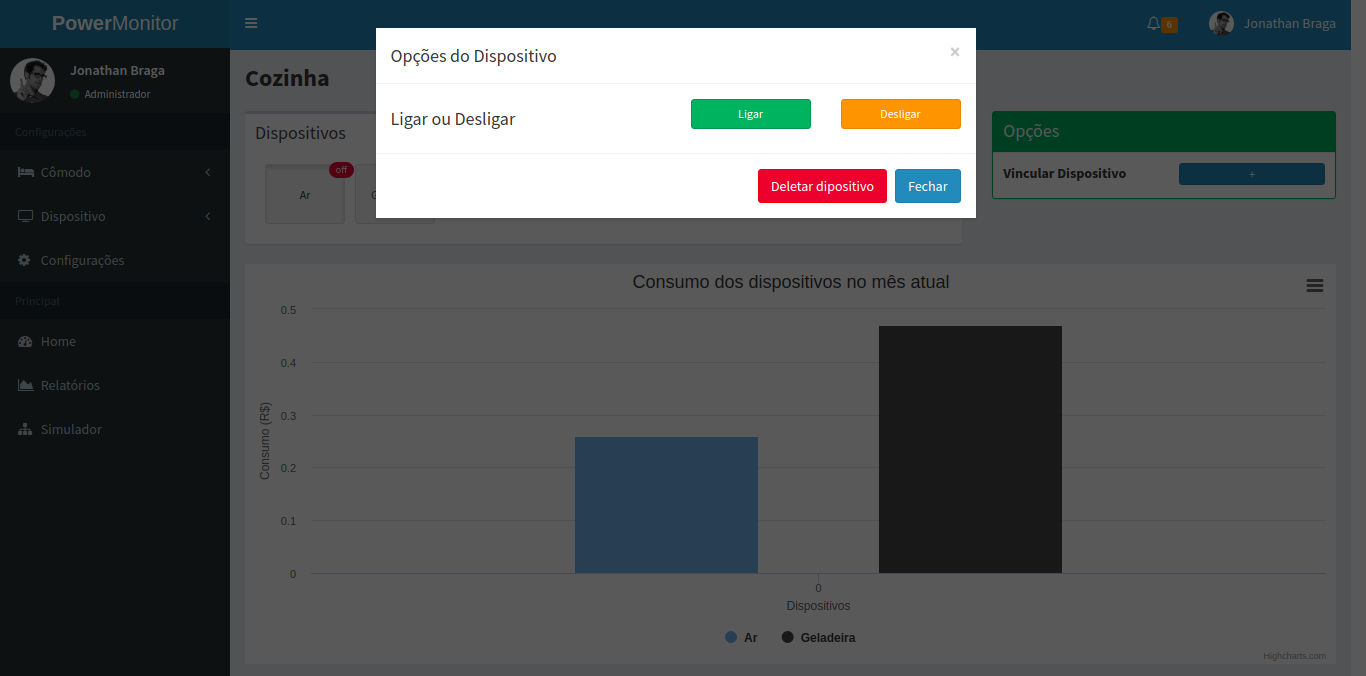
\includegraphics[width=1.0\textwidth, keepaspectratio=true]{a-dispositivo}
	\centering
	\caption[Ações que podem ser realizadas no dispositivo vinculado]{Ações que podem ser realizadas no dispositivo vinculado}
	\label{fig:a-dispositivo} 
\end{figure}
\FloatBarrier

Outras duas funcionalidades presentes no sistema são os alarmes gerados quando o usuário passa dos 50\% e dos 80\% do consumo esperado, cadastrado previamente pelo mesmo.
Também existe um simulador de gastos, onde é possível calcular o gasto mensal e diário que um dispositivo irá trazer para uma residência. As figuras
\ref{fig:aviso-a}, \ref{fig:aviso-v} e \ref{fig:simulador} retratam o descrito.

\begin{figure}[h!]
	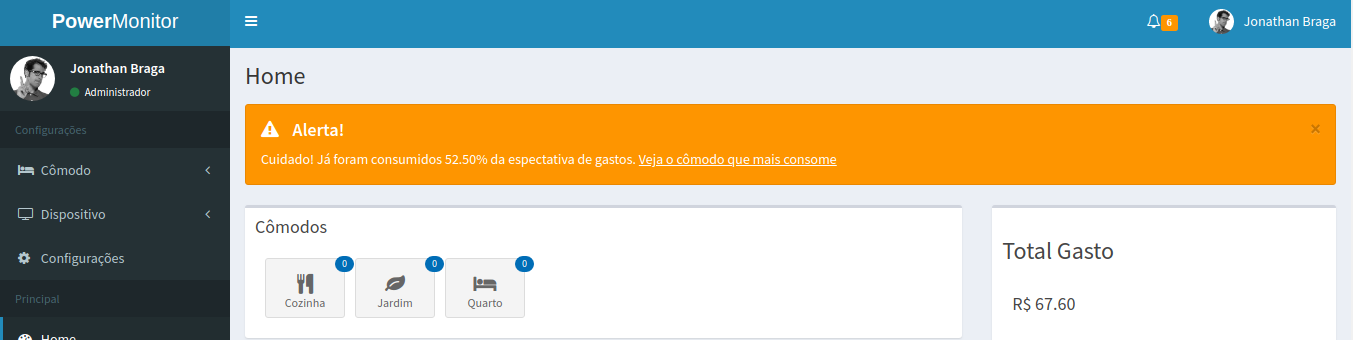
\includegraphics[width=1.0\textwidth, keepaspectratio=true]{aviso-a}
	\centering
	\caption[Alerta exibido quando o consumo supera os 50\% do previsto]{Alerta exibido quando o consumo supera os 50\% do previsto}
	\label{fig:aviso-a} 
\end{figure}
\FloatBarrier

\begin{figure}[h!]
	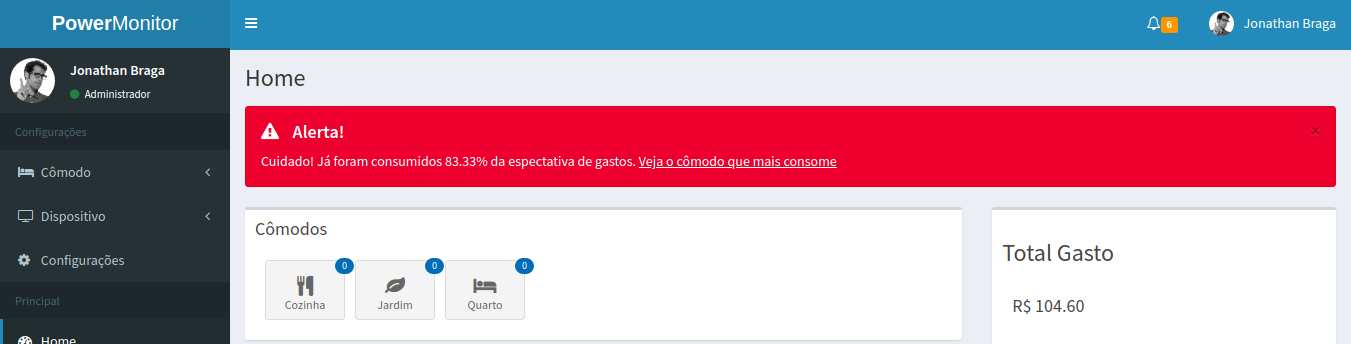
\includegraphics[width=1.0\textwidth, keepaspectratio=true]{aviso-v}
	\centering
	\caption[Alerta exibido quando o consumo supera os 80\% do previsto]{Alerta exibido quando o consumo supera os 80\% do previsto}
	\label{fig:aviso-v} 
\end{figure}
\FloatBarrier

\begin{figure}[h!]
	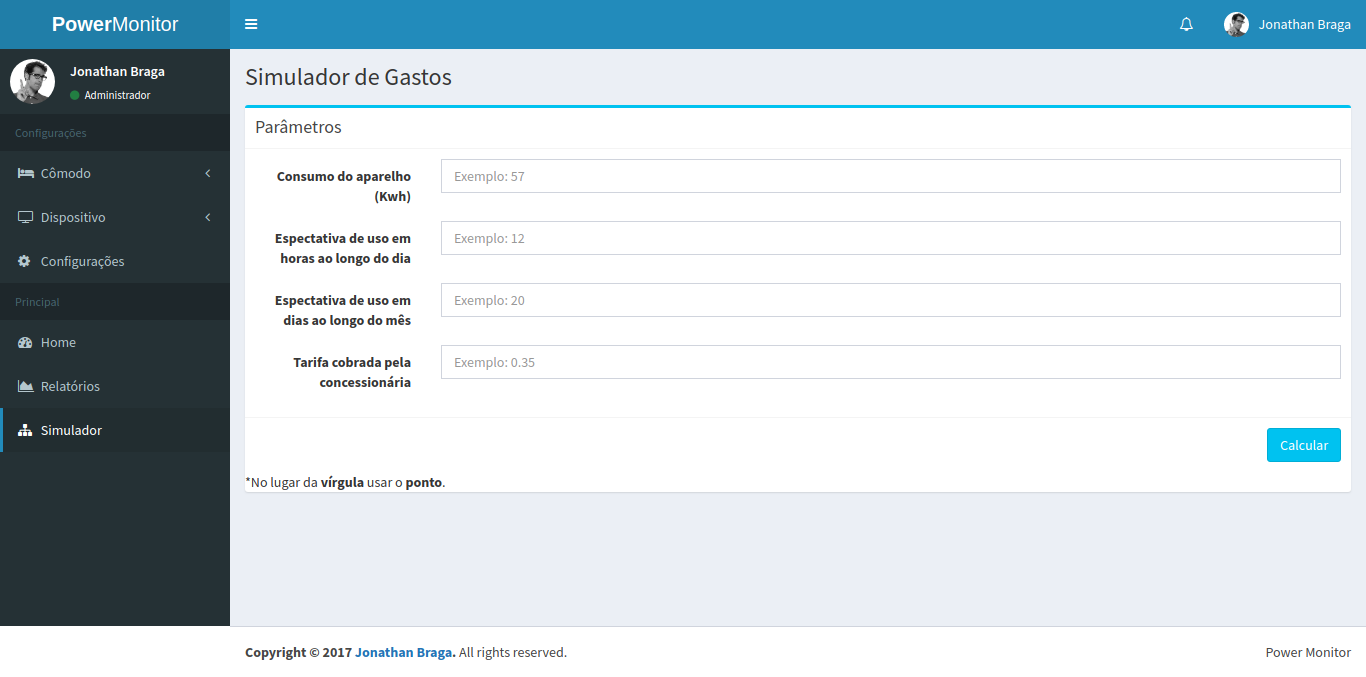
\includegraphics[width=1.0\textwidth, keepaspectratio=true]{simulador}
	\centering
	\caption[Simulador de gastos]{Simulador de gastos}
	\label{fig:simulador} 
\end{figure}
\FloatBarrier

\section[\textit{Hardware}]{\textit{Hardware}}\label{hard-sec}
O desenvolvimento do \textit{hardware} para demonstração da comunicação com o \textit{power monitor} envolve uma série de sensores e componentes
eletrônicos. A plataforma de prototipagem eletrônica utilizada para a construção desse \textit{hardware}, foi o NodeMCU(\autoref{esp}). O principal sensor
utilizado foi o SCT 013-000 (\autoref{sct}), que tem o papel de aferir dados da corrente que passa pelos dispositivos ao longo do tempo que o mesmo se encontra
ligado, também vale destacar o uso do relé que é responsável por toda a lógica de liga e desliga do dispositivo. O NodeMCU faz o intermédio da comunicação entre 
\textit{hardware} e servidor \textit{web}, fazendo toda a comunicação eletrônica entre o sensor e o circuito montado (\autoref{fig:circuito}), e enviando os dados
recebidos pelo sensor de corrente para o servidor \textit{web} que por sua vez, salva as medições aferidas no banco de dados. Com relação aos dados enviados 
para o banco, foi feito um algoritmo que ao identificar que o dispositivo está ligado verificando a corrente elétrica no presente momento e quando o mesmo é desligado 
é aferido novamente a corrente elétrica, esse resultado é multiplicado pelo valor da tensão
e assim é obtido o consumo do dispositivo (KWh). Após esse processo a informação é enviada via \textit{webscoket} 
para o servidor \textit{web} que salva tudo no banco de dados, e por fim a informação é consumida pela interface \textit{web}.

É válido lembrar que, para a comunicação \textit{websocket} é necessário o \textit{hardware} e o \textit{software} estarem conectados
na mesma rede \textit{Wi-Fi}. O grande motivo para a escolha do NodeMCU como plataforma de prototipagem foi a sua fácil comunicação com uma rede
\textit{Wi-Fi}, o código a seguir é um exemplo de como estabelecer a comunicação com uma rede sem fio.

\newpage

\begin{lstlisting}
	#include <NodeMCUWiFi.h>
	const char* ssid = NOME DA REDE;
	const char* password = SENHA;
	
	WiFi.begin(ssid, password);
\end{lstlisting}

Após estabelecer a conexão o próximo passo será interligar o servidor \textit{web} com o \textit{hardware} através da comunicação por \textit{websocket},
que será facilitada por meio da biblioteca \textit{SocketIOClient}, ela fornece alguns métodos como: \textit{\textbf{emit}}\protect\footnotemark, \textit{\textbf{on}}\protect\footnotemark 
e \textit{\textbf{connect}}\protect\footnotemark  que ajudam no momento de concretizar a comunicação total do \textit{hardware}. A seguir terá um
exemplo de como usar os métodos citados em conjunto com o código anterior.

\addtocounter{footnote}{-2}
\footnotetext{Função responsável por emitir os dados para o servidor \textit{web}}
\addtocounter{footnote}{1}
\footnotetext{Função responsável por receber os dados do servidor \textit{web}}
\addtocounter{footnote}{1}
\footnotetext{Função responsável por estabelecer conexão com servidor \textit{web}}

\begin{lstlisting}
	#include <SocketIOClient.h>
	SocketIOClient socket;
	const char* ssid = NOME DA REDE;
	const char* password = SENHA;
	String host = IP DO SERVIDOR WEB;
	int port = PORTA QUE FOI FORNECIDA AO SERVIDOR WEB;	

	void led(String state) {
	Serial.println("[led] " + state);
	if (state == "\"state\":true") {
	socket.emit("post-informacao","{\"data\":\"1\"}");
	}
	else {
	socket.emit("post-informacao","{\"data\":\"0\"}");
	}
	}

	void setup() {
		WiFi.begin(ssid, password);
  		socket.on("ligar", ligar);  
  		socket.connect(host, port);
	}

	void loop() {
  		socket.monitor();    
	}
\end{lstlisting}

A \autoref{fig:circuito} mostra bem o circuito demonstrativo utilizado neste trabalho para exemplificar a comunicação com o \textit{power monitor}.
O esquema representa uma forma prática e simples de se usar o sensor de corrente, o SCT 013-000 é ativado quando o usuário liga a lâmpada no interruptor
(representado por um botão) ou pelo sistema \textit{web} (\autoref{fig:a-dispositivo}), fazendo com que o relé ative e permita com que o dispositivo 
mude o estado para ligado. Após esse processo o sistema irá medir corrente que passa pelo dispositivo, e ao ser desligado o resultado
do consumo do dispositivo irá ser transmitido via \textit{websocket} para o servidor \textit{web} e se juntará com o resultado do tempo em que o dispositivo permaneceu
ligado para que por fim se possa se ter o consumo e o gasto deferido pelo equipamento. 

\begin{figure}[h!]
	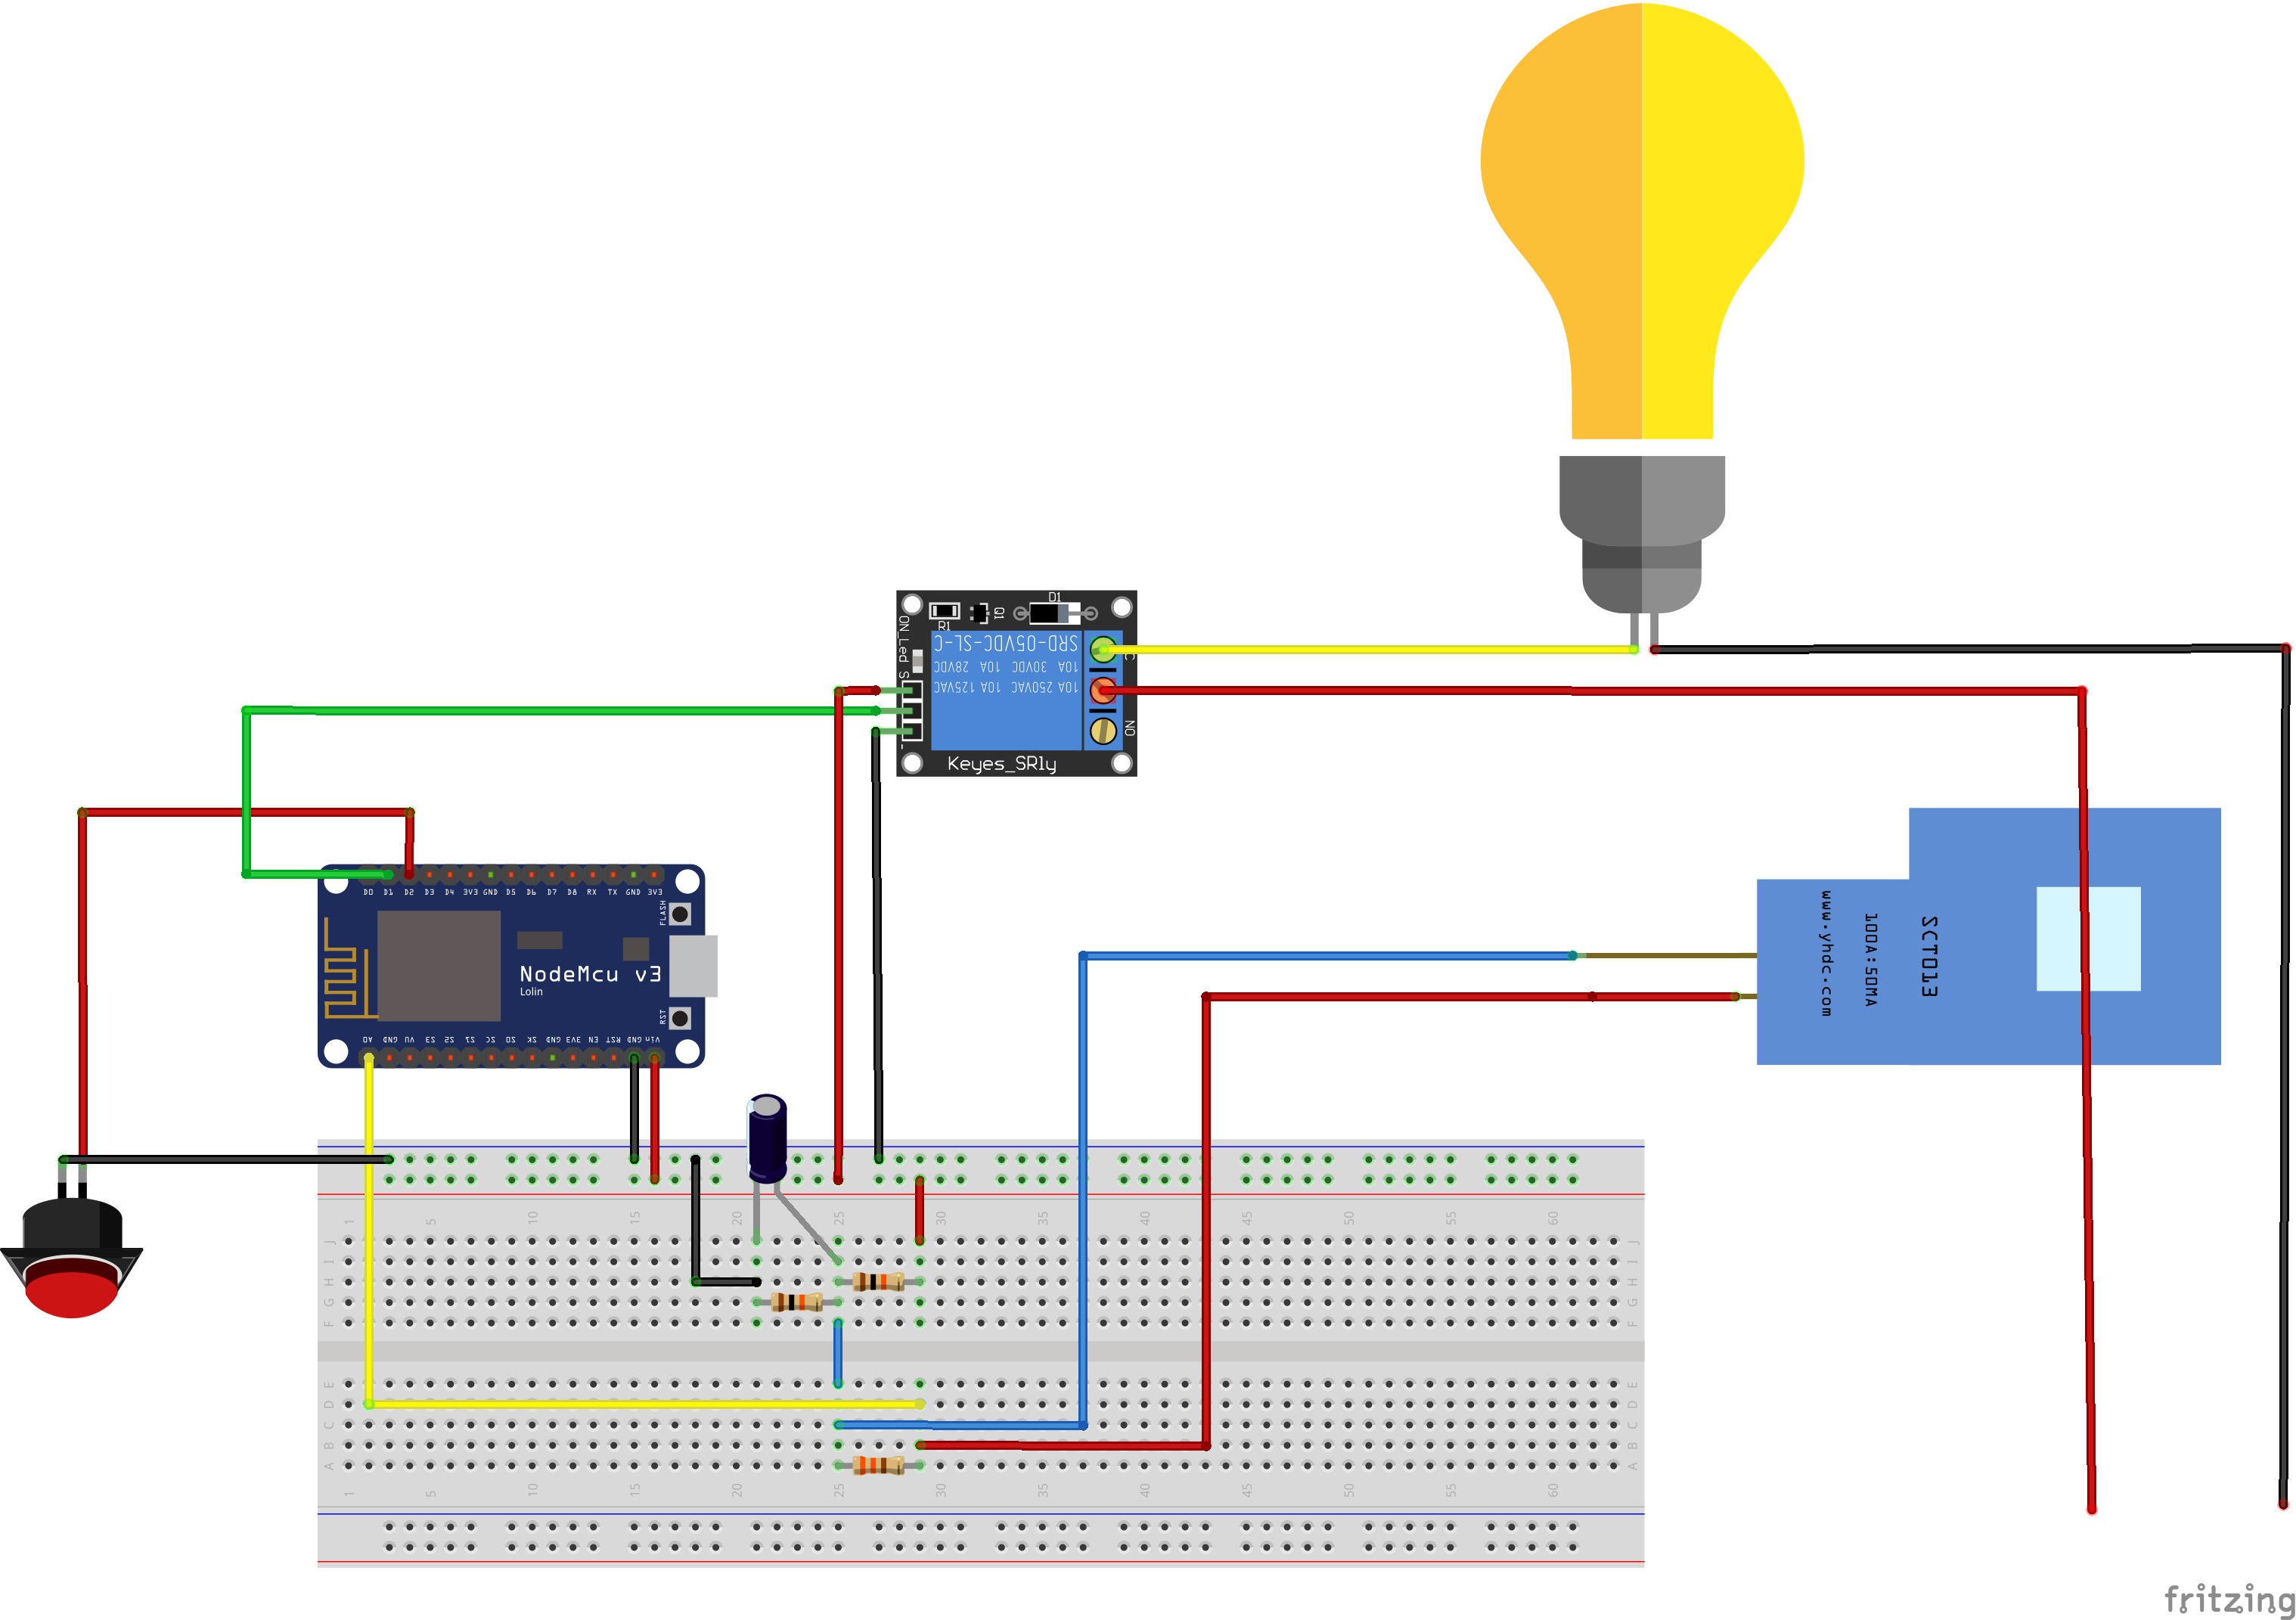
\includegraphics[width=0.8\textwidth, keepaspectratio=true]{circuito}
	\centering
	\caption[Circuito demonstrativo para comunicação com o \textit{power monitor}]{Circuito demonstrativo para comunicação com o \textit{power monitor}}
	\label{fig:circuito}  
\end{figure}
\FloatBarrier

\section[\textit{Resultados}]{\textit{Resultados}}\label{resultados-sec}

Depois de todo o estudo realizado, possibilidades discutidas e desenvolvimento detalhado, chegou-se ao  funcionamento da primeira versão
do \textit{softaware power monitor}. O sistema disponibiliza meios para uma fácil comunicação com qualquer \textit{hardware} de monitoramento
de energia e uma interface que leva o usuário a ter um novo entendimento e uma nova conscientização sobre o gasto energético. Trazendo uma forma menos
complicada de mensurar a quantidade de energia elétrica utilizada em uma residência, possibilitando também uma boa e simples leitura de quanto tem se gastado.

O \textit{power monitor} foi pensado para ser uma solução simples e barata, onde qualquer pessoa que tenha os devidos conhecimentos possa 
instalar, comunicar com \textit{hardwares} personalizados ou até mesmo modificar o código fonte. Como o \textit{software} foi desenvolvimento 
para que todos possam usar e modificar, todo o código fonte está disponível na plataforma de hospedagem de código fonte chamada 
\textit{GitHub} no seguinte endereço: \url{https://github.com/jonathanbraga/power-monitor}{}. A \autoref{custo-teste} mostra bem os 
custos do dispositivo que foram utilizados para a demonstração da comunicação com o \textit{power monitor}.


\begin{table}[!ht]
	\centering
	\begin{tabular}{ccc}
		\hline
		\textbf{Quantidade} & \textbf{Dispositivo}               & \textbf{Preço (R\$)}                 \\ \hline
		\rowcolor[HTML]{DDDDDD} 
		2                   & Resistor 10k$\Omega$ & 0,99                                 \\
		1                   & Resistor 330$\Omega$ & 0,99                                 \\
		\rowcolor[HTML]{DDDDDD} 
		1                   & Módulo Relé 5v                     & 9,00                                 \\
		1                   & NodeMCU                            & 59,76                                \\
		\rowcolor[HTML]{DDDDDD} 
		1                   & SCT 013-000                        & 58,80                                \\
		1                   & Capacitor eletrolítico 100uF       & 2,47                                 \\
		\rowcolor[HTML]{DDDDDD} 
		1                   & Conjunto de 40 Jumpers             & 9,00                                 \\
		1                   & Protoboard             & 20,00                                 \\
		1                   & Chave gangorra 2 terminais         & 3,00                                 \\ \hline
		\multicolumn{2}{|c|}{\textbf{TOTAL}}                     & \multicolumn{1}{c|}{\textbf{165,00}} \\ \hline
	\end{tabular}
	\caption{Custos do dispositivo de demonstração}
	\label{custo-teste}
\end{table} 